\chapter{Study Management}

This section first describes the study aggregate, its composition, and then
defines the commands it handles.

The \entitytarget{Study} aggregate is used to configure different aspects for a
study. It is used to define the valid types of specimens that can be collected
from participants, when they are to be collected, how the collected specimens
are processed, and allows for customization with use of annotation types. This
aggregate is made up of the entities and value objects shown in the figure
below.

\begin{figure}[H]
  \centering
  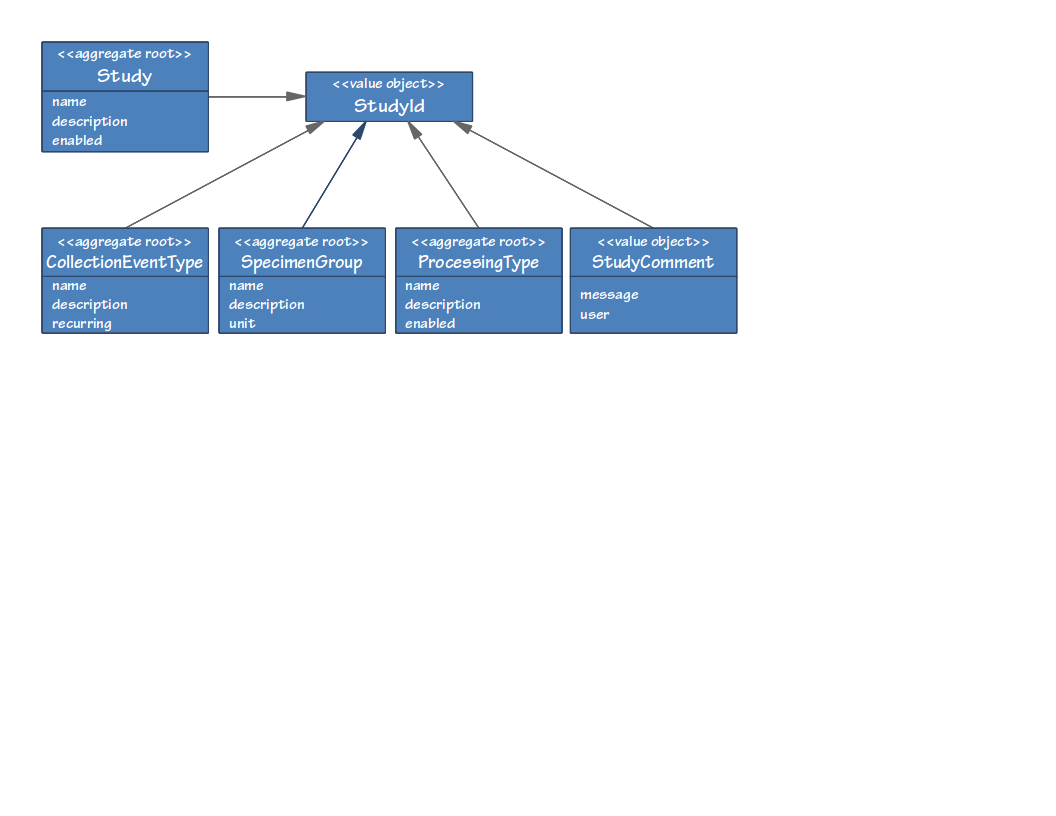
\includegraphics[trim={9mm 85mm 36mm 9mm}, clip,
    width=1\textwidth]{images/study-aggregate}
  \caption{Study aggregate}
  \label{fig:study-aggregate}
\end{figure}

\subsection*{Study}

A \entitylink{Study} represents a collection of participants and specimens
collected for a particular research study. Each study has a unique identifier,
\compfont{StudyId}, that is used to reference it. The \compfont{name} is a short
descriptive name, unique within the application, that is usually an acronym
used for quick identification.  The \compfont{description} give more details on
the name and is usually the words that make up the acronym.

A study can be enabled or disabled. When disabled, changes to its configuration
are possible but patients and specimens cannot be added. When enabled, no
further configuration changes are allowed, and participants and specimens can
be added.

As shown in the Figure \ref{fig:study-aggregate}, the study has collections of
other entities and value objects which are described below.

\subsection*{SpecimenGroup}

A \entitytarget{SpecimenGroup} is used to configure a specimen type used by the
study.  It records ownership, summary, storage, and classification information
that applies to an entire group or collection of \entitylink{Specimen}s. A
specimen group is defined either for specimens types collected from
participants, or for specimen types that are processed. More details for this
entity are given in Section \ref{sec:specimen-group}.

\subsection*{CollectionEventType}
A \entitytarget{CollectionEventType} defines a classification name, unique to
the \entitylink{Study}, to a paricipant visit. A participan visit is a record
of when specimens were collected from a participant at a collection
center. Each collection event type is assigned one or more specimen groups to
specify the specimen types that are collected. See Section
\ref{sec:collection-event-type} for more details.

\subsection*{ProcessingType}
A \entitytarget{ProcessingType} describes a regularly performed specimen
processing procedure with a unique name (unique to the
\entitylink{Study}). There should be one or more associated
\entitylink{SpecimenLinkType}s that (1) further define legal procedures and (2)
allow recording of procedures performed on different types of
\entitylink{Specimen}s. See Section \ref{sec:processing-type} for more details.

\subsection*{StudyAnnotationType}

\entitytarget{StudyAnnotationType}s allows a study to collect custom named and
defined pieces of data on collection event types (Section
\ref{sec:collection-event-type}), processing events (Section
\ref{sec:processing-type}), and participants (Section
\ref{sec:study-annotations}). Annotations are optional and are not a
requirement for specimen collection or processing.

\subsection*{StudyComment}
A \entitytarget{StudyComment} contains a textual message and the user that
added the comment. The date and time the comment was made is recorded as meta
data. A study can have one or more comments.

\section{SpecimenGroup Details}
\label{sec:specimen-group}

The \entitylink{SpecimenGroup} entity is composed of the value objects shown
in Figure \ref{fig:specimen-group}.

A specimen group has a name and an optional description. The name is a short
identifying name that is unique to the study, and the description can provide
additional details on the name. The unit specifies how the specimen amount is
measured (e.g. volume, weight, length, etc.).

A study can have one or more specimen groups. For specimen collection to be
allowed on a study, at least one specimen group must be defined.

\begin{figure}[H]
  \centering
  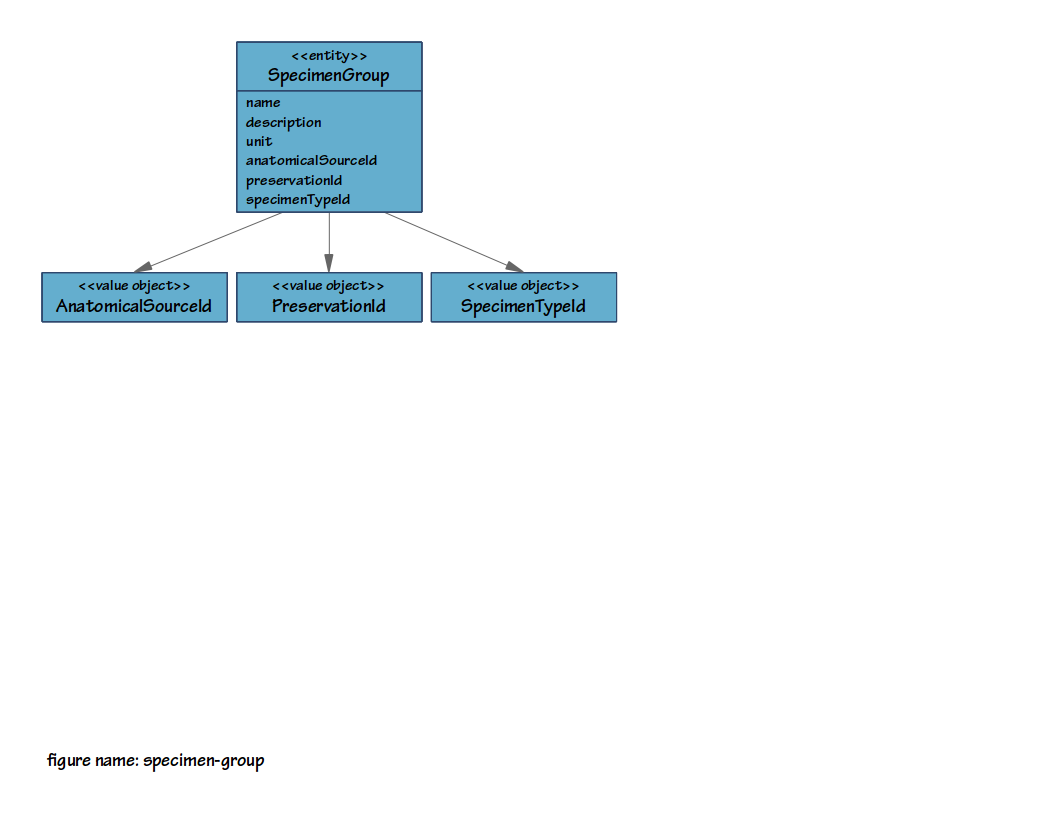
\includegraphics[trim={9mm 130mm 80mm 9mm}, clip,
    width=1\textwidth]{images/specimen-group}
  \caption{SpecimenGroup entity}
  \label{fig:specimen-group}
\end{figure}

\subsection*{AnatomicalSourceId}

An \valobjlink{AnatomicalSource} is a standardized set of regions from a
\entitylink{Participant} \emph{where} a \entitylink{Specimen} is collected
from. Potential examples include: colon, ear, leg, kidney,
etc. \valobjlink{AnatomicalSource} is a value object with a unique ID. They are
defined globally and new ones can be created at any time. They can be accessed
via look up service described in Section \ref{sec:lookup-service}.

A specimen group contains the ID of a single anatomical source.

\subsection*{PreservationId}

\valobjlink{Preservation} is a value object that describes how a
\entitylink{Specimen} should be preserved/stored by describing temperature
requirements ($^\circ$C), as well as a preservation method (see
\valobjlink{PreservationType}). \valobjlink{Preservation} is also a value
object with a unique ID. They are defined globally and new ones can be created
at any time. They can be accessed via look up service described in Section
\ref{sec:lookup-service}.

A specimen group contains the ID of a single preservation object.

\subsection*{SpecimenTypeId}

\valobjlink{SpecimenType} is standardized set of classifications that describe
\emph{what} a \entitylink{Specimen} is. Potential examples include: urine,
whole blood, plasma, nail, protein, etc. \valobjlink{SpecimenType} is also a
value object with a unique ID. They are defined globally and new ones can be
created at any time. They can be accessed via look up service described in
Section \ref{sec:lookup-service}.

A specimen group contains the ID of a single specimen type.

\section{CollectionEventType Details}
\label{sec:collection-event-type}
A collection event type has a name and an optional description. The name is a
short identifying name that is unique to the study, and the description can
provide additional details on the name. The \compfont{recurring} field is set to
\compfont{true} when the collection event type occurs more than once during the
lifetime of the study.

A collection event type can be configured to collect one or more specimens using
\entitylink{SpecimenGroupCollectionEventType}. It can also be configured to
record one or more annotation types using
\entitylink{CollectionEventTypeAnnotationType}. These associations are shown in
Figure \ref{fig:collection-event-type}.

A study can have one or more collection event types defined. For specimen
collection to be allowed on a study, at least one collection event type must be
defined.

\begin{figure}[H]
  \centering
  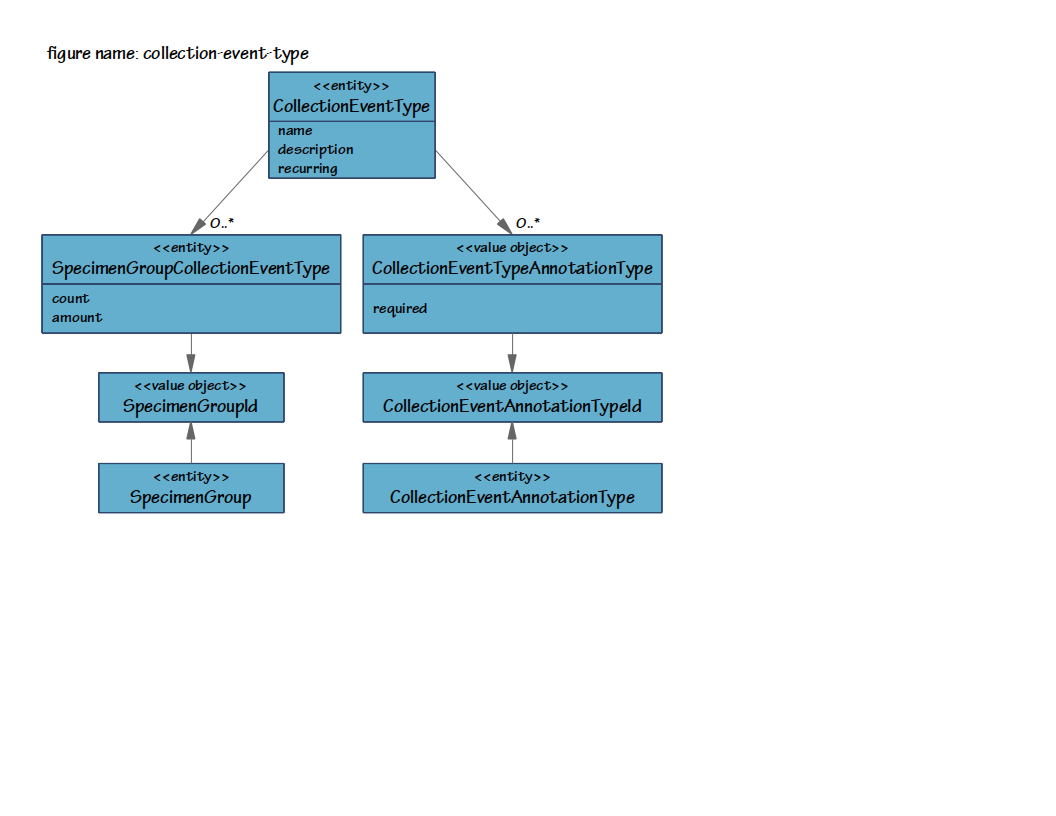
\includegraphics[trim={9mm 65mm 96mm 9mm}, clip,
    width=0.8\textwidth]{images/collection-event-type}
  \caption{Details for the CollectionEventType entity}
  \label{fig:collection-event-type}
\end{figure}

\subsection*{SpecimenGroupCollectionEventType}

\valobjtarget{SpecimenGroupCollectionEventType}s are used to define which types
of specimens (i.e. which \valobjlink{SpecimenGroup}s) need to be collected with
a type of collection event. A single specimen group can be used in multiple
collection event types.

The \compfont{count} specifies how many specimens are to be collected. The
\compfont{amount} is the amount of substance that is expected in each collected
specimen, or null if there is no default amount. The unit on the amount is
defined in the \entitylink{SpecimenGroup}.

\subsection*{CollectionEventAnnotationType}

Collection event annotations are defined using
\valobjtarget{CollectionEventAnnotationType}. One or more of these can be
defined for the study. A single collection event annotation type can be used in
multiple collection event types. When \compfont{required} is set to
\compfont{true}, the annotation value is not allowed to be empty.

\section{ProcessingType Details}
\label{sec:processing-type}

A processing type has a name and an optional description. The name is a short
identifying name that is unique to the study, and the description can provide
additional details on the name. A processing type should have \compfont{enabled}
set to \compfont{true} when processing of the contained specimen types is taking
place. However, throughout the lifetime of the study, it may be decided to stop
a processing type in favour of another. In this case \compfont{enabled} is set to
\compfont{false}.

A processing type can be configured to process one or more collected specimens
using \valobjlink{SpecimenLinkType}. Individual specimen link types within the
processing type can also be configured to record one or more annotation using
\valobjlink{SpecimenLinkTypeAnnotationType}. Figure \ref{fig:processing-type}
provides more details for the processing type entity.

One or more processing types can be defined for a study. For specimen
processing to be allowed on a study, at least one processing type must be
defined.

\begin{figure}[H]
  \centering
  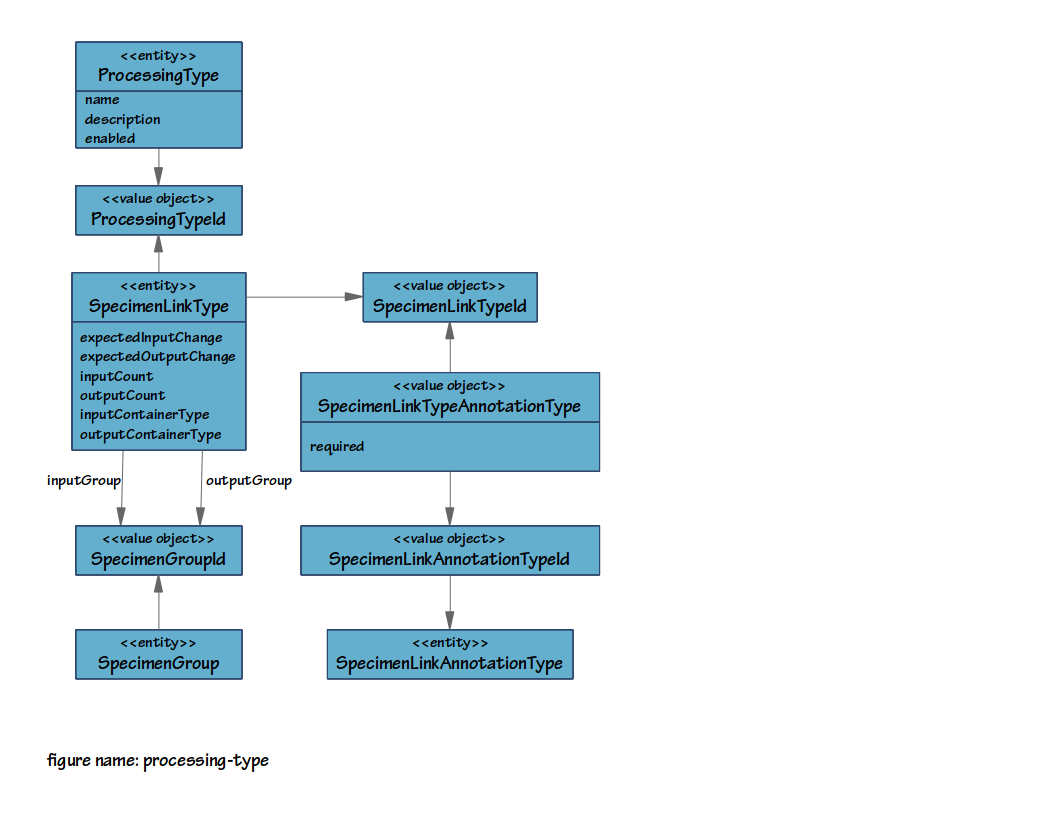
\includegraphics[trim={9mm 35mm 120mm 9mm}, clip,
    width=0.7\textwidth]{images/processing-type}
  \caption{Details for the ProcessingType entity.}
  \label{fig:processing-type}
\end{figure}

Processing of specimens is not allowed until at least one processing type is
defined for the study.

\subsection*{SpecimenLinkType}

 \valobjtarget{SpecimenLinkType}s are assigned to
a processing type, and used to represent a regularly performed processing
procedure involving two \entitylink{Specimen}s: an input, which must be in a
specific \valobjlink{SpecimenGroup}, and an output, which must be in a specific
\valobjlink{SpecimenGroup}.

The \compfont{expectedInputChange} is the expected amount (decimal value) to be
removed from each input. The \compfont{expectedOutputChange} (also a decimal
value) is the expected amount to be added to each output. If the expected input
and output change values are not required, they can be assigned a zero value.
The counts in \compfont{inputCount} and \compfont{outputCount} are the number of
expected and resulting specimens, respectively, when the processing is carried
out. A value of zero for output count implies that the count is the same as the
input count. The specimen container type that holds the input specimens is
given in \compfont{inputContainerType}. The specimen container type that the
output specimens are stored into is given in \compfont{outputContainerType}. If
specifying the container types is not required for one or both of these fields,
they can be assigned a \compfont{null} value.

To avoid redundancy, a specimen link type may exist only once for a given input
and output specimen group.

\subsection*{SpecimenLinkTypeAnnotationType}

A \valobjtarget{SpecimenLinkTypeAnnotationType} is used to tie a specimen
link annotation type to a specimen link type.

\section{Study Annotations}
\label{sec:study-annotations}

Figure \ref{fig:study-annotations} show the possible annotations types that can
be configured for a study. Annotations types must be defined before they can be
assigned to the respective entity. See Chapter \ref{chap:annotations} for more
details on how annotations are configured and used.

\begin{figure}[H]
  \centering
  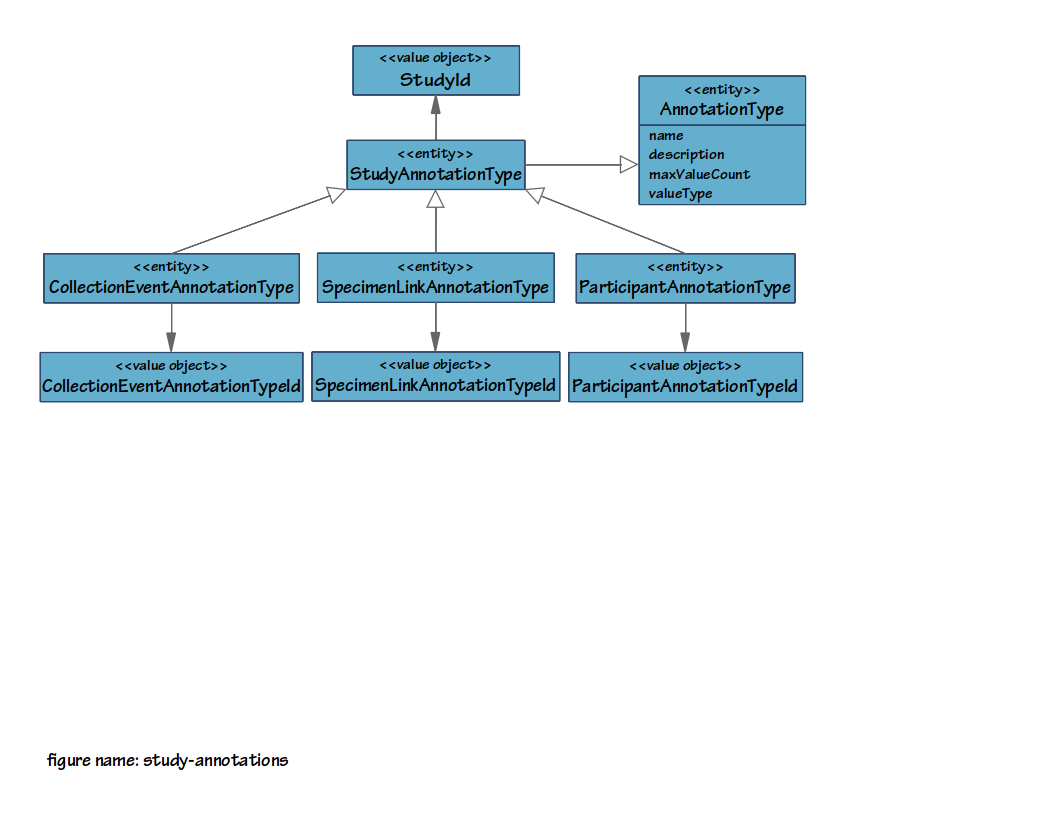
\includegraphics[trim={9mm 135mm 68mm 9mm}, clip,
    width=0.9\textwidth]{images/study-annotations}
  \caption{Study annotation entities}
  \label{fig:study-annotations}
\end{figure}

\subsection*{CollectionEventTypeAnnotationType}

A \entitytarget{CollectionEventTypeAnnotationType} is used to to configure an
annotation to be used by collection event types. An example of an annotation on
a collection even type can be consent given by the participant at the
collection visit. \valobjtarget{CollectionEvent

\subsection*{SpecimenLinkAnnotationType}

A \valobjtarget{SpecimenLinkAnnotationType} is used to to configure an
annotation to be used with specimen link types.

An example of an annotation type on a specimen link can be the PMBC count on
the collected specimen.

\subsection*{ParticipantAnnotationType}

A \valobjtarget{ParticipantAnnotationType} is used to to configure a an
annotation for a participant. When \compfont{required} is set to true the
annotation value is not allowed to be empty.

An example of an annotation on a participant can be their gender.

\section {Study Aggregate Commands}

\subsection{Study Commands}
The commands handled by the study aggregate are listed below.

\subsection*{CreateStudyCommand}

Creates a new study. A study can be created at any time. If a study with the
given name already exists the command fails and throws a checked exception.

\begin{commandparmtable}

  name & string & A short descriptive name associated with the study. Usually
  an acronym.\\

  description & string & A more detailed name for the study. If an acronym is
  used for the study name, then the description should contain the words that
  make up the acronym.\\

\end{commandparmtable}

\subsection*{UpdateStudyCommand}

Update a study's name, description, or both. If a study with the
new name already exists the command fails and throws a checked exception.

\begin{commandparmtable}

  studyId & string & The study's unique identifier.\\

  name & string & The new name, or the original name if it's not being modified.\\

  description & string & The new description, or the original description if
  it's not being modified.\\

\end{commandparmtable}

\subsection*{EnableStudyCommand}

Enables a study. Once enabled the study is ready to collect and process
specimens from participants.

\begin{commandparmtable}

  studyId & string & The study's unique identifier.\\

\end{commandparmtable}

\subsection*{DisableStudyCommand}

Used to disable a study. A study may be disabled because no more specimen
collection and processing will be done on it, or because it requires
configuration changes. Once disabled specimen collection and processing cannot
be performed on this study.

\begin{commandparmtable}

  studyId & string & The study's unique identifier.\\

\end{commandparmtable}

\subsection{Specimen Group Commands}
\subsection*{CreateSpecimenGroupCommand}

Creates a specimen group on a study. If the study is not disabled the command
fails and throws a checked exception. If a specimen group already exists with
the given name the command fails and throws a checked exception.

\begin{commandparmtable}

  studyId & string & The study's unique identifier.\\

  name & string & A short descriptive name.\\

  description & string & Provides more details for the specimen group. Can be left empty.\\

  anatomicalSourceId & string & The ID corresponding to the anatomical source this group
  belongs to.\\

  preservationId & string & The ID corresponding to the preservation used by this
  specimen group.\\

  specimenTypeId & string & The ID corresponding to the specimen type.\\

\end{commandparmtable}

\subsection*{UpdateSpecimenGroupCommand}

Updates a specimen group on a study. If the study is not disabled the command
fails and throws a checked exception. If a specimen group already exists with
the new name the command fails and throws a checked exception.

\begin{commandparmtable}

  studyId & string & The study's unique identifier.\\

  name & string & The new name, or the original name if it's not being modified.\\

  description & string & The new description, or the original description if
  it's not being modified.\\

  anatomicalSourceId & string & The ID corresponding to the updated or original
  anatomical source.\\

  preservationId & string & The ID corresponding to the updated or original preservation.\\

  specimenTypeId & string & The ID corresponding to the updated or original specimen type.\\

\end{commandparmtable}

\subsection*{DeleteSpecimenGroupCommand}

Deletes a specimen group from the study. If the study is not disabled the
command fails and throws a checked exception.

\begin{commandparmtable}

  studyId & string & The study's unique identifier.\\

  specimenGroupId & string & The specimen group's unique identifier.\\

\end{commandparmtable}
% Local Variables:
% compile-command: "/usr/bin/rubber --pdf main"
% End:


\subsection{Collection Event Type Commands}

\subsection*{CreateCollectionEventType}
Creates a collection event type for a study. If the study is not disabled the
command fails and throws a checked exception. The command fails with a checked
exception if name already exists.
\begin{commandparmtable}

  studyId & string & The study's unique identifier.\\

  name & string & A short descriptive name.\\

  description & string & Provides more details. Can be left empty.\\

  recurring & boolean & Set to \compfont{true} if this collection event type
  occurs more than once for the duration of the study.\\

\end{commandparmtable}

\subsection*{UpdateCollectionEventType}
Updates one or more attributes of a collection event type. If a collection event with the
given name already exists the command fails and throws a checked exception.
\begin{commandparmtable}

  studyId & string & The study's unique identifier.\\

  collectionEventTypeId & string & The collection event type's unique identifier.\\

  name & string & The new name, or the original name if it's not being modified.\\

  description & string & The new description, or the original description if
  it's not being modified.\\

  recurring & boolean & The new value, or the original value if it's not being
  modified.\\

\end{commandparmtable}

\subsection*{DeleteCollectionEventType}
Deletes a collection event type.
\begin{commandparmtable}

  studyId & string & The study's unique identifier.\\

  collectionEventTypeId & string & The collection event type's unique identifier.\\

\end{commandparmtable}

\subsection*{AddSpecimenGroupToCollectionEventType}
Adds a specimen group to a collection event type.
\begin{commandparmtable}

  studyId & string & The study's unique identifier.\\

  collectionEventTypeId & string & The collection event type's unique identifier.\\

  specimenGroupId & string & The specimen group's unique identifier.\\

\end{commandparmtable}

\subsection*{RemoveSpecimenGroupFromCollectionEventType}
Removes a specimen group from a collection event type.
\begin{commandparmtable}

  studyId & string & The study's unique identifier.\\

  collectionEventTypeId & string & The collection event type's unique identifier.\\

  specimenGroupId & string & The specimen group's unique identifier.\\

\end{commandparmtable}

\subsection*{AddAnnotationToCollectionEventType}
Adds an annotation type to a collection event type.

\begin{commandparmtable}

  studyId & string & The study's unique identifier.\\

  collectionEventTypeId & string & The collection event type's unique identifier.\\

  collectionEventAnnotationTypeId & string & The annotation type's unique identifier.\\

\end{commandparmtable}

\subsection*{RemoveAnnotationFromCollectionEventType}
Removes an annotation type from a collection event type.

\begin{commandparmtable}

  studyId & string & The study's unique identifier.\\

  collectionEventTypeId & string & The collection event type's unique identifier.\\

  collectionEventAnnotationTypeId & string & The annotation type's unique identifier.\\

\end{commandparmtable}
% Local Variables:
% compile-command: "/usr/bin/rubber --pdf main"
% End:


\subsection{Processing Type Commands}

\subsection*{CreateProcessingType}
Creates a processing type for a study. If the study is not disabled the command
fails and throws a checked exception. The command fails with a checked
exception if name already exists.

\begin{commandparmtable}

  studyId & string & The study's unique identifier.\\

  name & string & A short descriptive name.\\

  description & string & Provides more details. Can be left empty.\\

  enabled & boolean & Set to \texttt{true} when this processing type is still
  in use.\\

\end{commandparmtable}

\subsection*{UpdateProcessingType}
Updates one or more attributes of a processing type. If a processing with the
given name already exists the command fails and throws a checked exception.

\begin{commandparmtable}

  studyId & string & The study's unique identifier.\\

  processingTypeId & string & The processing type's unique identifier.\\

  name & string & The new name, or the original name if it's not being modified.\\

  description & string & The new description, or the original description if
  it's not being modified.\\

  enabled & boolean & The new value, or the original value if it's not being
  modified.\\

\end{commandparmtable}

\subsection*{DeleteProcessingType}
Deletes a processing type.

\begin{commandparmtable}

  studyId & string & The study's unique identifier.\\

  processingTypeId & string & The processing type's unique identifier.\\

\end{commandparmtable}

\subsection*{EnableProcessingType}
Used to enable a processing type that was previously disabled.

\begin{commandparmtable}

  studyId & string & The study's unique identifier.\\

  processingTypeId & string & The processing type's unique identifier.\\

\end{commandparmtable}

\subsection*{DisableProcessingType}
Used to disable a processing type that was previously enabled.

\begin{commandparmtable}

  studyId & string & The study's unique identifier.\\

  processingTypeId & string & The processing type's unique identifier.\\

\end{commandparmtable}

\subsection*{AddSpecimenLinkType}

\begin{commandparmtable}

  studyId & string & The study's unique identifier.\\

  processingTypeId & string & The processing type's unique identifier.\\

  expectedInputChange & decimal & Amount to be removed from input. Use a value
  of zero if amount change tracking is not required.\\

  expectedOutputChange & decimal & Amount to be added to each output. Use a value
  of zero if amount change tracking is not required.\\

  inputCount & integer & The number of expected specimens.\\

  outputCount & integer & The number of resulting specimens after processing. A
  value of zero implies that the output count is the same as the input count.\\

  inputContainerType & \entitylink{SpecimenContainer} & The specimen container type
  that holds the input specimens.\\

  outputContainerType & \entitylink{SpecimenContainer} & The specimen container type
  that holds the output specimens.\\

\end{commandparmtable}

\subsection*{UpdateSpecimenLinkType}

\begin{commandparmtable}

  studyId & string & The study's unique identifier.\\

  processingTypeId & string & The processing type's unique identifier.\\

  specimenLinkTypeId & string & The specimen link type's unique identifier.\\

  expectedInputChange & decimal & The new or original input change amount.\\

  expectedOutputChange & decimal & The new or original output change amount.\\

  inputCount & integer & The new or original number expected specimens.\\

  outputCount & integer & The new or original number of resulting specimens.\\

  inputContainerType & \entitylink{SpecimenContainer} & The new or original
  input specimen container type.\\

  outputContainerType & \entitylink{SpecimenContainer} & The new or original
  output specimen container type.\\

\end{commandparmtable}

\subsection*{RemoveSpecimenLinkType}

\begin{commandparmtable}

  studyId & string & The study's unique identifier.\\

  processingTypeId & string & The processing type's unique identifier.\\

  specimenLinkTypeId & string & The specimen link type's unique identifier.\\

\end{commandparmtable}

\subsection*{AddInputSpecimenGroupToSpecimenLinkType}

\begin{commandparmtable}

  studyId & string & The study's unique identifier.\\

  processingTypeId & string & The processing type's unique identifier.\\

  specimenLinkTypeId & string & The specimen link type's unique identifier.\\

  specimenGroupId & string & The specimen group's unique identifier.\\

\end{commandparmtable}

\subsection*{RemoveInputSpecimenGroupFromSpecimenLinkType}

\begin{commandparmtable}

  studyId & string & The study's unique identifier.\\

  processingTypeId & string & The processing type's unique identifier.\\

  specimenLinkTypeId & string & The specimen link type's unique identifier.\\

  specimenGroupId & string & The specimen group's unique identifier.\\

\end{commandparmtable}

\subsection*{AddOutputSpecimenGroupToSpecimenLinkType}

\begin{commandparmtable}

  studyId & string & The study's unique identifier.\\

  processingTypeId & string & The processing type's unique identifier.\\

  specimenLinkTypeId & string & The specimen link type's unique identifier.\\

  specimenGroupId & string & The specimen group's unique identifier.\\

\end{commandparmtable}

\subsection*{RemoveOutputSpecimenGroupFromSpecimenLinkType}

\begin{commandparmtable}

  studyId & string & The study's unique identifier.\\

  processingTypeId & string & The processing type's unique identifier.\\

  specimenLinkTypeId & string & The specimen link type's unique identifier.\\

  specimenGroupId & string & The specimen group's unique identifier.\\

\end{commandparmtable}

\subsection*{AddAnnotationToSpecimenLinkType}

\begin{commandparmtable}

  studyId & string & The study's unique identifier.\\

  processingTypeId & string & The processing type's unique identifier.\\

  specimenLinkTypeId & string & The specimen link type's unique identifier.\\

  specimenLinkAnnotationTypeId & string & The specimen link annotation types's
  unique identifier.\\

  required & boolean & Use \texttt{true} when this annotation type is required
  and cannot be left empty.\\

\end{commandparmtable}

\subsection*{RemoveAnnotationFromSpecimenLinkType}

\begin{commandparmtable}

  studyId & string & The study's unique identifier.\\

  processingTypeId & string & The processing type's unique identifier.\\

  specimenLinkTypeId & string & The specimen link type's unique identifier.\\

  specimenLinkAnnotationTypeId & string & The specimen link annotation types's
  unique identifier.\\

\end{commandparmtable}

\subsection{Study Annotations}

The commands for adding a collection event type - annotation types are shown
here. The commands to add annotations to \entitylink{SpecimenLink} and
\entitylink{Participants} as similar to these commands but are not listed here.

See the \entitytarget{AddAnnotationOption} command for adding annotation
options to \texttt{SELECT} annotation types.

\subsection*{CreateCollectionEventTypeAnnotationType}

\begin{commandparmtable}
  studyId & string & The study's unique identifier.\\

  name & string & A short descriptive name.\\

  description & string & Provides more details. Can be left empty.\\

  valueType & \valobjlink{AnnotationValueType} & The types of values
  (e.g. string, number, date, etc.) this type of annotation expects.\\

  maxValueCount & integer & If value type is \texttt{SELECT}, then this is the
  maximum number of selections that can be made. Use zero for unlimited.\\
\end{commandparmtable}

\subsection*{UpdateCollectionEventTypeAnnotationType}

\begin{commandparmtable}
  studyId & string & The study's unique identifier.\\

  collectionEventAnnotationTypeId & string & The annotation type's unique identifier.\\

  name & string & The updated or original name.\\

  description & string & The updated or original description.\\

  valueType & \valobjlink{AnnotationValueType} & The updated or original value type.\\

  maxValueCount & integer & The updated or original count.\\
\end{commandparmtable}

\subsection*{DeleteCollectionEventTypeAnnotationType}

\begin{commandparmtable}
  studyId & string & The study's unique identifier.\\

  collectionEventAnnotationTypeId & string & The annotation type's unique identifier.\\
\end{commandparmtable}

\subsection*{AddCollectionEventTypeAnnotationOptions}
The command fails if the annotation value type is not \texttt{SELECT}.

\begin{commandparmtable}
  studyId & string & The study's unique identifier.\\

  collectionEventAnnotationTypeId & string & The annotation type's unique
  identifier.\\

  options & Set[String] & The options to add for this annotation.\\
\end{commandparmtable}


% Local Variables:
% compile-command: "/usr/bin/rubber --pdf main"
% End:

